% !TEX root = ../main_final_en.tex
\section{Pipeline Implementation}

The development and evaluation of the predictive models were carried out entirely in \textbf{Python}, using \texttt{scikit-learn}, \texttt{cuML}, \texttt{PyTorch} and the \textit{gradient boosting} libraries \texttt{XGBoost}, \texttt{LightGBM} and \texttt{CatBoost}. Models trained exclusively with IFN3 data were run on a local machine (Intel Core i7, 32~GB RAM), while those using IFN2 and IFN3 data jointly were trained on the high-performance computing (HPC) system of the University of Salamanca, leveraging Nvidia H100 graphics cards to accelerate the training of GPU-compatible models.

\subsection{Feature selection}\label{sec:seleccion_variables}

\subsubsection{Manual selection}

The manual feature selection started from a thematic organisation of the predictor set, grouping variables according to the type of ecological, structural or climatic information they represent. This classification allowed the dimensionality reduction process to be structured around the following conceptual blocks:

\begin{itemize}
    \item \textbf{Fixed variable block}: describes the basic structure of the forest stand and the essential identification and general characterisation attributes of each plot.
    \item \textbf{Species variable block}: collects information on the composition, state and specific characteristics of the forest formations.
    \item \textbf{Substrate block}: integrates edaphic and management variables susceptible to change over time.
    \item \textbf{Terrain block}: groups physical properties of the medium that remain stable at the temporal scale of inventories (slope, aspect, soil type, etc.).
    \item \textbf{Summary climatic block}: represented by the Martonne aridity index, which synthesises the interaction between temperature and precipitation.
    \item \textbf{Detailed climatic block}: includes explicit seasonal metrics for temperature and precipitation.
    \item \textbf{Vegetation index block}: collects spectral information related to water status, vigour and photosynthetic activity of the vegetation.
\end{itemize}

In total, the database initially contained 445 candidate variables distributed among these thematic blocks. After applying the manual selection procedure, supported by statistical, ecological and model performance comparison criteria, the set was reduced to 44 representative variables. The variables finally selected within each block were:

{%
\renewcommand{\_}{\textunderscore\discretionary{}{}{}}%
\begin{itemize}
    \item \textbf{Fixed variable block}:
          \texttt{especie\_id}, \texttt{tipo\_especie}, \texttt{grupo\_id}, \texttt{periodo}, \texttt{radio}, \texttt{ocupa},
          \texttt{npies\_1}, \texttt{npies\_2}, \texttt{npies\_5},
          \texttt{npies\_10}, \texttt{npies\_15}, \texttt{npies\_20},
          \texttt{npies\_25}, \texttt{npies\_30}, \texttt{npies\_35},
          \texttt{npies\_40}, \texttt{npies\_45}, \texttt{npies\_50},
          \texttt{npies\_55}, \texttt{npies\_60}, \texttt{npies\_65},
          \texttt{npies\_70}.

    \item \textbf{Species variable block}:
          \texttt{estado\_id}, \texttt{fccarb}, \texttt{disesp\_id}.

    \item \textbf{Substrate block (dynamic)}:
          \texttt{modcomb\_id}, \texttt{nivel2\_id},
          \texttt{tratmasa\_id}.

    \item \textbf{Terrain block}:
          \texttt{rocosidad\_id},
          \texttt{orientacion\_cat}, \texttt{elevacion}, \texttt{pendiente\_cat}.

    \item \textbf{Summary climatic block (Martonne)}:
          \texttt{martonneidx\_id}.

    \item \textbf{Detailed climatic block (temperature and precipitation)}:
          \texttt{skt\_mean\_primavera}, \texttt{skt\_mean\_verano},
          \texttt{skt\_std\_primavera}, \texttt{skt\_std\_verano},
          \texttt{pr\_sum\_invierno}, \texttt{pr\_sum\_otoño},
          \texttt{pr\_sum\_primavera}, \texttt{pr\_sum\_verano}.

    \item \textbf{Vegetation index block}:
          \texttt{gndvi\_mean\_verano}, \texttt{ndii\_mean\_primavera},
          \texttt{gndvi\_std\_primavera}, \texttt{evi\_mean\_primavera}.
\end{itemize}
}%

The comparison of models trained with incremental combinations of blocks showed that all of them contribute relevant information, following the approximate order of contribution: \textit{fixed variables} $>$ \textit{species variables} $>$ \textit{substrate} $>$ \textit{terrain} $>$ \textit{vegetation indices} $>$ \textit{Martonne} $>$ \textit{temperature and precipitation}. That is, most of the predictive capacity is explained by the structure and composition of the forest stand, while edaphic, topographic and climatic conditions act as additional modulators of carbon accumulation.

\subsubsection{Automatic selection}

\textit{Featurewiz} selected \textbf{67 variables}, with preference for vegetation indices derived from Sentinel-2 (NDII, EVI, GNDVI and NDVI, with mean, maximum, minimum, median and standard deviation statistics, especially in spring and summer) and seasonal thermal and precipitation variables (\texttt{t2m\_*}, \texttt{skt\_*}, \texttt{stl\_*}, \texttt{pr\_sum\_*}, \texttt{pr\_max\_*}, \texttt{pr\_min\_*}). The Martonne aridity index and a representative set of structural variables (trees per diameter class), species and terrain variables completed the selection.

\textit{mRMR} selected \textbf{50 variables} prioritising high mutual information with carbon and low internal redundancy. The set integrates structural predictors (species, radius, diameter classes, aspect and slope), edaphic variables (rockiness, soil types), seasonal climatic metrics and seasonal means of NDII, GNDVI and EVI, confirming that photosynthetic activity and water status act as direct predictors of stored carbon.

\subsubsection{Selection result}
Of the three selected variable sets, the manual selection was retained as it demonstrated better performance with greater simplicity.

\subsection{\textit{Stacking} configuration}

Aggregation via \textit{stacking} was implemented with out-of-fold (OOF) predictions generated on the training set with the same \texttt{GroupKFold} scheme; each base model was retrained on the entire training set to produce the final predictions on test. The meta-variables were standardised using \texttt{StandardScaler} before fitting the meta-model.

With the aim of studying the trade-off between ensemble diversity, computational cost and performance, five base model configurations were defined (Table~\ref{tab:stack_configs}). BayesianNN, SVR and MLP models were discarded as candidates due to their lower individual performance.

\begin{table}[htbp]
  \centering
  \caption{\textit{Stacking} base model configurations.}
  \label{tab:stack_configs}
  \resizebox{\columnwidth}{!}{%
  \begin{tabular}{cp{6cm}}
    \toprule
    \textbf{Config.} & \textbf{Base models} \\
    \midrule
    1 & LightGBM, Random Forest \\
    2 & LightGBM, XGBoost, GBDT \\
    3 & CatBoost, Random Forest, GBDT \\
    4 & CatBoost, LightGBM, Random Forest,\newline GBDT \\
    5 & CatBoost, LightGBM, XGBoost,\newline Random Forest, GBDT, BaggedDT \\
    \bottomrule
  \end{tabular}}
\end{table}

The configurations range from the lightest (Config.~1, two models with different paradigms) to the most complete (Config.~5, all models with competitive performance), allowing the effect of structural diversity and computational cost on ensemble performance to be analysed. On the stacked predictions of each configuration, the meta-models listed in Table~\ref{tab:meta_modelos} were trained.

\begin{table}
    \centering
    \caption{Meta-models used in \textit{stacking} together with their parameters.}
    \label{tab:meta_modelos}
    \footnotesize
    \resizebox{\columnwidth}{!}{
    \begin{tabular}{m{3.5cm}m{5cm}}
        \toprule
        \textbf{Meta-model} & \textbf{Parameters} \\
        \midrule
        Gradient Boosting   & Default configuration \\
        Linear Regression    & No regularisation \\
        Ridge               & L2 regularisation with cross-validation ($\alpha \in \{0.01, 0.1, 1, 10, 100\}$) \\
        Random Forest       & 50 trees \\
        SVR                 & Linear kernel \\
        MLP                 & One hidden layer with 50 neurons, 500 maximum iterations \\
        \bottomrule
    \end{tabular}
    }
\end{table}

By evaluating all combinations of base model configurations with the different meta-models, a set of ensembles is obtained that allow a systematic study of which subsets of base models are most complementary and which type of meta-model best exploits the information contained in their predictions.


\subsection{Final training data}
\label{subsec:datos_finales_entrenamiento}

After applying the eligibility and filtering criteria described in
Section~\ref{subsec:filtradoregistros}, the final dataset used
for model fitting consists of:

\begin{itemize}
    \item \textbf{IFN2:} Total plots = \textbf{88,696}
          \begin{itemize}
              \item Cases with $c4 > c$: \textbf{41,761}
              \item Cases with $carbono\_bruto4 > carbono\_bruto$: \textbf{43,539}
          \end{itemize}

    \item \textbf{IFN3:} Total plots = \textbf{171,157}
          \begin{itemize}
              \item Cases with $fccarb \geq 20$: \textbf{164,364}
              \item Cases with $fccarb \geq 20$ and $c4 > c$: \textbf{62,029}
              \item Cases with $fccarb \geq 20$ and $carbono\_bruto4 > carbono\_bruto$: \textbf{89,580}
          \end{itemize}
\end{itemize}

Table~\ref{tab:descriptivos} summarises the main descriptive statistics of the target variables used in the modelling.
It can be observed that the variable \texttt{carbono\_bruto4} has a mean of 20.79 and a standard deviation of 35.09, while the variable \texttt{c4} shows notably higher values (mean of 38.83 and standard deviation of 47.27). A histogram of the distribution of the target variables can be found in Figure \ref{fig:histograma_datos_combinado}.


\begin{table}[htbp]
  \centering
  \caption{Descriptive statistics of the cleaned dataset.}
  \label{tab:descriptivos}
  \resizebox{\columnwidth}{!}{%
  \begin{tabular}{lrrrrr}
    \toprule
    \textbf{Variable} & \textbf{N} & \textbf{Mean} & \textbf{Std. dev.} & \textbf{Min.} & \textbf{Max.} \\\\
    \midrule
    carbono\_bruto4 & 133\,119 & 20.79 & 35.09 & 0.00 & 420.50 \\
    carbono\_bruto & 123\,563 & 10.09 & 26.33 & 0.00 & 511.31 \\
    c4 & 103\,790 & 38.83 & 47.27 & 0.48 & 883.46 \\
    c & 131\,942 & 29.58 & 40.62 & 0.44 & 873.36 \\
    \bottomrule
  \end{tabular}}
\end{table}




\begin{figure}
    \centering
    \begin{subfigure}{0.48\textwidth}
        \centering
        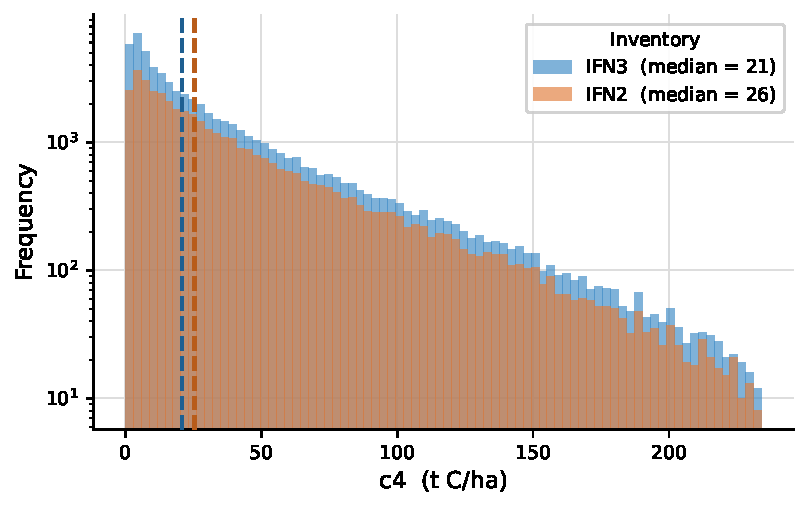
\includegraphics[width=\textwidth]{figuras/06_desarrollo_modelo/hist_c4.pdf}
        \caption{Histogram of the \texttt{c4} variable on a logarithmic scale.}
        \label{fig:hist_c4_sub}
    \end{subfigure}
    \hfill
    \begin{subfigure}{0.48\textwidth}
        \centering
        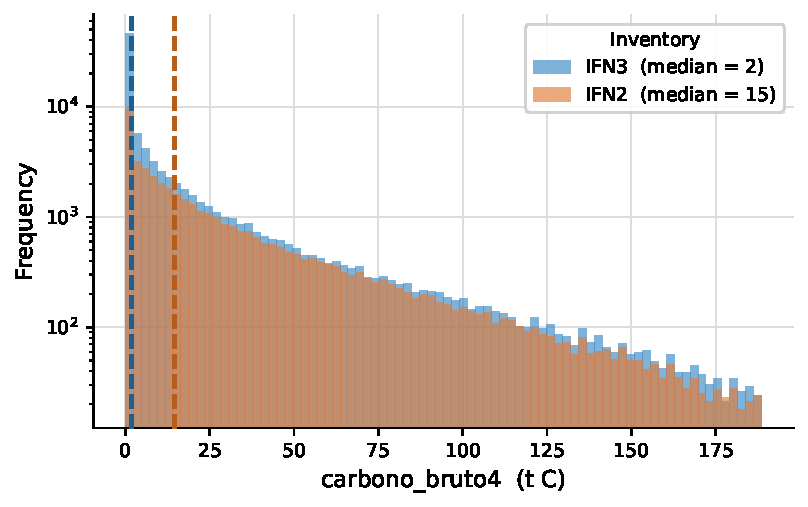
\includegraphics[width=\textwidth]{figuras/06_desarrollo_modelo/hist_carbono_bruto4.pdf}
        \caption{Histogram of the \texttt{carbono\_bruto4} variable on a logarithmic scale.}
        \label{fig:hist_carbono_bruto4_sub}
    \end{subfigure}
    \caption{Histogram of the \texttt{c4} and \texttt{carbono\_bruto4} variables in the cleaned dataset.}
    \label{fig:histograma_datos_combinado}
\end{figure}

On the other hand, Figure \ref{fig:distribucion_variables_combinado} shows the distributions of the target variables separated by inventory. It can be observed that the histogram of the \texttt{carbono\_bruto4} variable is notably more concentrated at low values than that corresponding to \texttt{c4}, for which the amount of carbon has been standardised per unit area.

\begin{figure}
    \centering
    \begin{subfigure}{0.48\textwidth}
        \centering
        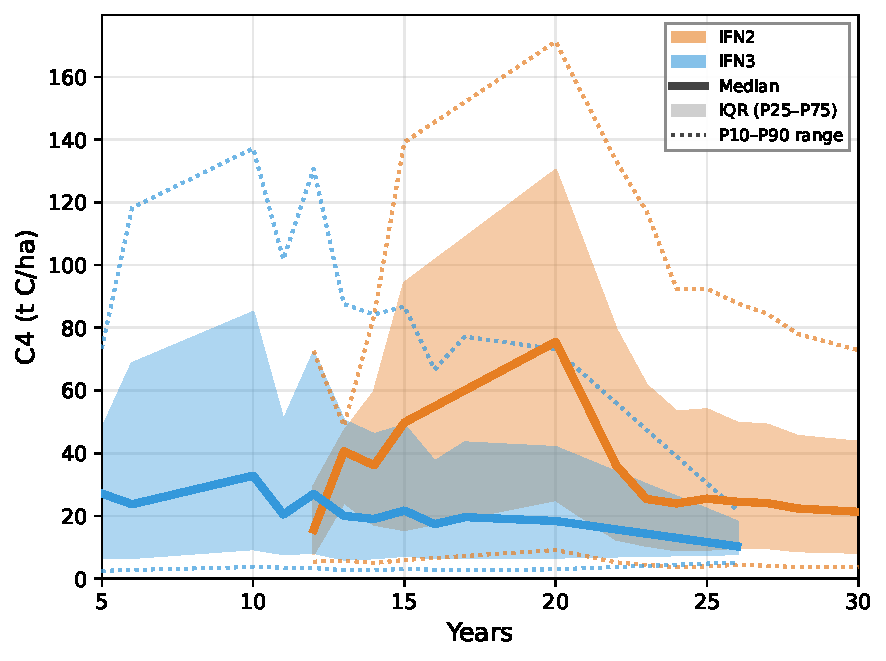
\includegraphics[width=\textwidth]{figuras/06_desarrollo_modelo/ribbon_c4.pdf}
        \caption{Distribution of the \texttt{c4} variable across values of the \texttt{periodo\_agrupado} variable.}
        \label{fig:distribucion_c4_sub}
    \end{subfigure}
    \hfill
    \begin{subfigure}{0.48\textwidth}
        \centering
        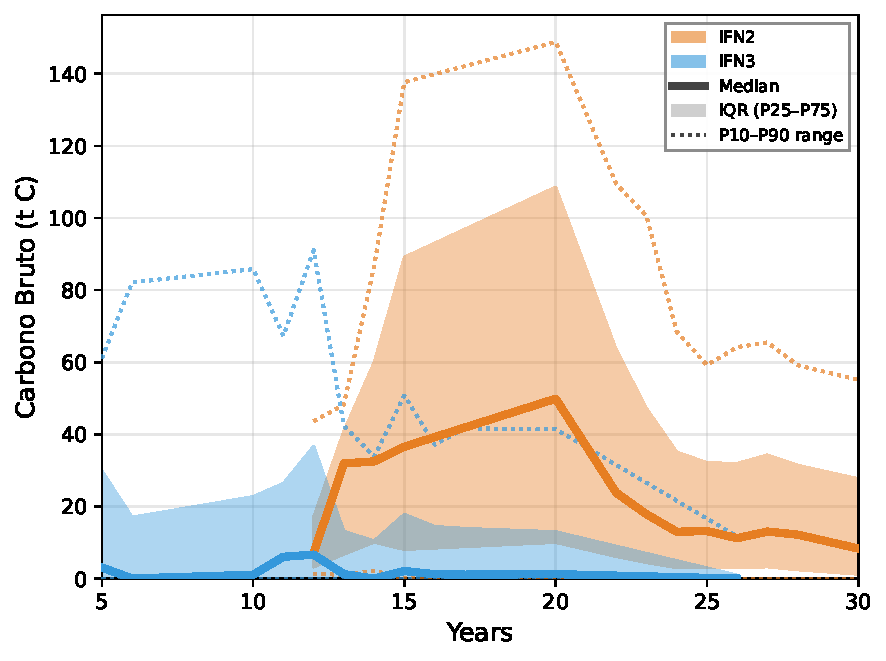
\includegraphics[width=\textwidth]{figuras/06_desarrollo_modelo/ribbon_carbono_bruto4.pdf}
        \caption{Distribution of the \texttt{carbono\_bruto4} variable across values of the \texttt{periodo\_agrupado} variable.}
        \label{fig:distribucion_carbono_bruto4_sub}
    \end{subfigure}
    \caption{Distribution of the \texttt{c4} and \texttt{carbono\_bruto4} variables in the cleaned dataset (after applying filters) separated by inventory.}
    \label{fig:distribucion_variables_combinado}
\end{figure}


\subsubsection{Effect of the period on carbon}
\label{subsec:resultados_periodo_anova}

The influence of \textit{periodo} on the carbon variables was evaluated
using one-way ANOVA. The analyses carried out
show that \textit{periodo} has a significant effect on both
variables. For \texttt{c4}, a test statistic of
\(F = 143.49\) \((p < 0.001)\) was obtained, while for \texttt{carbono\_bruto4}
the value was \(F = 161.08\) \((p < 0.001)\).
These results indicate that the differences observed between periods
are not random, but reflect systematic variations associated with the
sampling time, confirming that \textit{periodo} constitutes a
relevant explanatory factor in the dynamics of forest carbon.
